\section{Stanford CoreNLP}
\label{sec:stanfordparser}

Die Stanford \ac{NLP} Group, ein Team aus Software- und Linguistik Experten, entwickelt quelloffene Software zur Anwendung von \ac{NLP}. Resultat dieser Entwicklung ist eine Menge von Programmen, die jeweils eigenständige \ac{NLP} Probleme lösen und als Software mit eigener Distribution verfügbar sind (\cite[vgl.][1 ff.]{STANFORDNLPTEAM}).  Darunter befindet sich der Stanford Parser. Dieser ist, neben anderen Modulen, aber auch Bestandteil der Stanford CoreNLP Suite, einer seit 2010 offen verfügbaren, vereinigten Distribution der verschiedenen \ac{NLP} Komponenten mit einheitlicher Schnittstelle (\cite[vgl.][1 ff.]{STANFORDNLP}). Das grundlegende Prinzip des Stanford CoreNLPs besteht darin, den zu analysierenden Text in einzelne Elemente, also etwa Worte, zu zerlegen und diese mit Meta-Annotationen verschiedener funktionaler Komponenten zu versehen.\par
Dieses Kapitel soll eine Auswahl derartiger, einzelner Komponenten des Stanford CoreNLP und ihre Funktionsweise grundlegend erläutern. Zu diesem Zweck wird bei einigen dieser Er\-läu\-ter\-ung\-en eine Analyse-Visualisierung folgenden Minimalbeispiels verwendet:
\begin{quote}
"'The student writes his paper at the DHBW. After he is finished, he hands it in."'
\end{quote} Diese Visualisierung wird jeweils anhand eines Web-Tools der Stanford \ac{NLP} Group vorgenommen.\footnote{Erreichbar unter: http://nlp.stanford.edu:8080/corenlp/} Weiterhin soll die Verwendung des Stanford CoreNLP Toolkits mit Java thematisiert werden. Außerdem sei an dieser Stelle angemerkt, dass der von Friedrich im State-Of-The-Art Ansatz verwendete Stanford Parser lediglich über die beiden in Abschnitt \ref{subsec:pos} und \ref{subsec:parser} erläuterten Funktionen verfügt.
\newpage
\subsection{Part-of-Speech}
\label{subsec:pos}

\begin{wrapfigure}{r}{8cm}
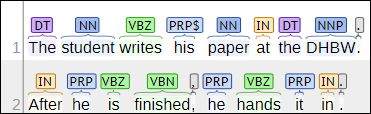
\includegraphics[width=8cm]{pictures/POS.png}
\caption{Visualisierung der POS am Beispiel}
\label{fig:POS}
\end{wrapfigure}

Als \ac{POS} wird die Art eines Wortes bezeichnet. Ein Wort kann beispielsweise ein Nomen, Verb oder Adjektiv sein. Das Stanford CoreNLP über eine Funktionalität, die \ac{POS} Annotationen zu den einzelnen Worten des analysierten Texts hinzufügt.\par
Zu diesem Zweck werden vorhergehende und folgende Wörter im jeweiligen Satz betrachtet. Realisiert wird diese Funktionalität über ein Dependency-Network (\cite[vgl.][1]{POSTAGGER}), das auf die \textit{Penn Treebank} angewandt wird. Dabei handelt es sich um eine Datenbank von syntaktisch analysiertem Text. Abbildung \ref{fig:POS} zeigt das mit POS-Tags versehene Beispiel. Jedes einzelne Wort, wird einer Wortart anhand einer Abkürzung zugeordnet. Beispielsweise steht der dem Wort "'student"' zugeordnete Tag "'NN"' für \textit{Noun}. Der POS-Tagger unterscheidet die 36 verschiedenen Wortarten der Penn Treebank (\cite[vgl.][3]{PENNTREEBANK}), die in Tabelle \ref{table:POSTAGS} vollständig aufgelistet sind.

\subsection{Parser}
\label{subsec:parser}
\begin{wrapfigure}{r}{8cm}
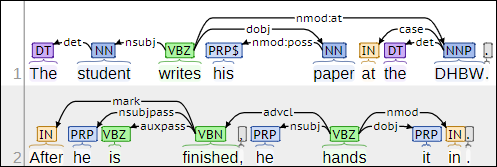
\includegraphics[width=8cm]{pictures/Parser.png}
\caption{Visualisierung der Erweiterten Abhängikeiten am Beispiel}
\label{fig:ENHDEPS}
\end{wrapfigure}
Der Parser des Stanford CoreNLPs baut auf den POS-Tags auf und liefert eine nochmals erweiterte syntaktische Analyse des Textes. Es werden zusätzlich zusammengehörige Phrasen im Satz ermittelt. Dafür werden wiederum zwei unterschiedliche Repräsentationen unterstützt (\cite[vgl.][4]{STANFORDNLP}). Die Analyse kann zum einen durch Abhängigkeiten, zum anderen durch den Aufbau wiedergegeben werden. Diese Abhängigkeiten eines bestimmten Typs werden gerichtet zwischen zwei Worten gebildet. Eine Vollständige Liste aller Abkürzungen der Abhängigkeitstypen findet sich in Anhang A.2. Die Notation der Analyse nach dem Aufbau erfolgt hingegen anhand einer Baumstruktur. Der Text wird hierbei in Phrasen-Typen eingeteilt und die einzelnen Worte diesen zugeordnet.\par Es existieren verschiedene Implementierungsstrategien für den Stanford Parser. Im Stanford CoreNLP wird ein Ansatz anhand eines Neuronalen Netzes verfolgt, der entsprechend auf Wahrscheinlichkeiten basiert. Dieser zeichnet sich vor Allem durch die Realisierung performanter Ausführungszeiten bei einer präzisen Vorhersagegenauigkeit aus (\cite[vgl.][8]{DEPPARSER}).\par
Abbildung \ref{fig:ENHDEPS} zeigt die Syntaktische Analyse anhand der Abhängigkeiten innerhalb der beiden Beispielsätze. So existiert etwa eine Abhängigkeit des Typs det (determiner) vom Wort "'student"' zum Wort "'the"'. Die Schlussfolgerung ist, dass diese beiden Worte eine inhaltliche Phrase bilden und es sich bei "'the"' um einen Artikel handelt.

\subsection{Named-Entity-Recognition}
\label{subsec:ner}
\begin{wrapfigure}{r}{8cm}
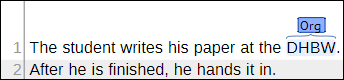
\includegraphics[width=8cm]{pictures/NER.png}
\caption{Visualisierung der NER am Beispiel}
\label{fig:NER}
\end{wrapfigure}
Ein Bestandteil natürlicher Sprache ist die Erwähnung von Eigennamen etwa bestimmter Orte, Personen oder auch Organisationen. Daher verfügt das Stanford CoreNLP über die \ac{NER}. Mit Hilfe dieser Funktionalität können derartige Wörter erkannt und in Bezug auf die Entität, welche sie bezeichnen,  klassifiziert werden. Zu diesem Zweck existieren die vier Kategorien person (PER), location (LOC), organization (ORG) und miscellaneous (MISC) (\cite[vgl.][4]{STANFORDNER}).\par
Beispielsweise könnte ein Wort mit der Annotation "'ORG"' versehen werden, was darauf hinweist, dass es sich dabei um den Namen einer Organisation handelt. So zeigt Abbildung \ref{fig:NER}, dass die Bezeichnung "'DHBW"' im Beispielsatz von der \ac{NER} als Organisation erkannt wird.\par
Zur Implementierung dieses Features wurde eine lexikalische Datenbasis verwendet, weswegen letztlich nicht alle Namen als solche erkannt werden können. Werden bestimmte, mit der \ac{NER} nicht klassifizierbare Namen im Text erwartet, können diese auch regelbasiert anhand eines frei definierbaren Regulären Ausdrucks identifiziert werden (REGEXNER).

\subsection{Coreference Resolution}
\label{subsec:coref}
\begin{wrapfigure}{r}{8cm}
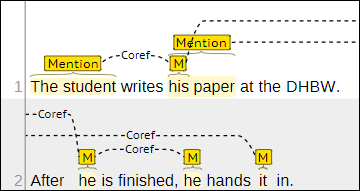
\includegraphics[width=8cm]{pictures/coref.png}
\caption{Visualisierung der Coreference Resolution am Beispiel}
\label{fig:COREF}
\end{wrapfigure}
Ein Text in natürlicher Sprache bezieht sich auf Entitäten nicht nur anhand deren eigentlicher Bezeichnung. In der Regel werden diese Bezeichnungen in derartigen Bezügen auch durch Pronomina o.Ä. ersetzt. Dies kann insbesondere auch satzübergreifend geschehen. Das Stanford CoreNLP ermöglicht über die Coreference Resolution eine Auflösung der Beziehungen zwischen den bezeichneten Entitäten und ihren jeweiligen substitutiven Elementen. Die Implementierung basiert auf einer Kombination aus regelbasierten und Machine Learning Algorithmen, die als deterministischer Ansatz beschrieben wird (\cite[vgl.][1]{COREFERENCE}).\par
Abbildung \ref{fig:COREF} zeigt die Bezüge der Pronomina zu ihren jeweiligen Entitäten über beide Sätze des Beispiels hinweg.  So beziehen sich etwa die Worte "'he"' und "'it"' im zweiten Satz jeweils auf die Worte "'student"' und "'paper"'.

\subsection{Sentiment Analysis}
\label{subsec:sentiment}
Neben reinem Inhalt verfügt ein Satz in natürlicher Sprache auch über eine Stimmung. Diese äußert sich vorrangig anhand der Auswahl der Worte und deren Konnotation. Das Stanford CoreNLP bietet daher die Sentiment Analysis. Hiermit können Sätze bezüglich ihrer Stimmung als "'negativ"', "'neutral"' oder "'positiv"' annotiert werden.\par
Umgesetzt wird diese Funktionalität unter Anwendung eines rekursiven Neuronalen Netzes, also eines Deep Learning Algorithmus. Zum Training des Netzes wurde die "'Stanford Sentiment Treebank"' verwendet,eine Sammlung von Begriffen versehen mit der jeweiligen Konnotation (\cite[vgl.][1]{SOCHERSENTIMENT}).

\subsection{Java API}
\label{subsec:corenlpjava}
Alle Funktionen des Stanford CoreNLP können unter einem einheitlichen \ac{API} adressiert werden, welches ursprünglich für die Verwendung unter Java konzipiert wurde. Jedoch existieren auch Implementierungen für andere Sprachen, wie etwa Python, Ruby oder Scala (\cite[vgl.][3]{STANFORDNLP}). Es soll weiterhin die grundlegende Funktionsweise dieser \ac{API} erläutert werden.\par
Die Basis dafür bildet ein Annotation-Objekt, welches reinen Text als Eingabe akzeptiert und nach Ausführung einen annotierten Text ausgibt. Ein mögliches Ausgabeformat für den Annotierten Text ist unter anderem XML. Die funktionalen Module des Stanford CoreNLP, wovon die meisten in diesem Kapitel bereits erkäutert wurden, werden über Annotater repräsentiert. Diese werden sequentiell auf den Text angewendet und fügen Annotationen hinzu. Im Konstruktor des Annotation-Objekts können die gewünschten Annotater über einen String spezifiziert werden (\cite[vgl.][1]{STANFORDNLP}).\par
Weiterhin besteht die Möglichkeit eigene Logik anhand eigener Annotator auszuführen. Hierzu muss ein Interface implementiert werden und der Name der Klasse angegeben. Die Instanzierung erfolgt wie bei den Standard Klassen durch den String des Annotation-Konstruktors über class-reflection (\cite[vgl.][4]{STANFORDNLP}).

\subsection{Weitere Standard NLP-Tookits}

Neben dem Stanford CoreNLP gibt es noch zwei weitere weit verbreitete Standards. Das \ac{NLTK} ist eine Sammlung von Programmmodulen zur Verarbeitung von natürlicher Sprache. Ebenso wie beim Stanford CoreNLP handelt es sich um einen Standard Bibliothek, die grundlegende \ac{NLP} Aufgaben abdeckt. Das \ac{NLTK} steht unter der \textit{GLP Open Source Licence} und wurde für die Programmiersprache Pyhon entwickelt. Es greift auf diverse lexikalische Ressourcen wie WordNet, FrameNet aber auch Wikipedia zurück. Das \ac{NLTK} verfügt im Gegensatz zum Stanford CoreNLP über einfach handhabbare Visualisierungsmodule. Das StanfordCoreNLP kann zwar in Python, das NLTK aber nicht in Java verwendet werden.
\par
Eine weitere Alternative stelle das Apache Projekt OpenNLTK dar. Die Java-Bibliothek ist Machine Learning basiert und erfüllt ebenfalls die gängigen NLP Aufgaben.

